\chapter{Related work}
\label{chapter:related}

\section{An in-depth look to ``Human-level control through deep reinforcement learning'' paper}
This section is dedicated to analyzing the paper which is proposes a method for solving games using deep learning and reinforcement learning. The proposed agent, called Q-Network capable of playing 43 different games and adapting to each one without being modified.


\begin{figure}[h]
	\floatname{algorithm}{Algorithm}
	\begin{center}
		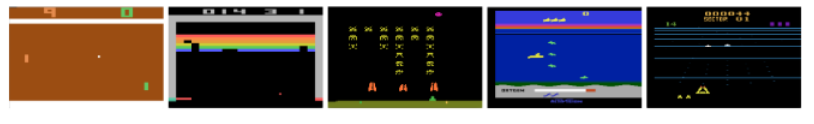
\includegraphics[width=334px,height=51px]{src/img/state/ataripic}
		\caption{Snapshots with five Atari 2600 Games: Pong, Breakout, Space Invaders, Seaquest, Beam Rider\cite{nature}} \label{fig:ataripic}
    \end{center}
\end{figure}




\section{Architecture}
The article\cite{nature} proposes a new type of network, Q-network which combines convolutional layers, a representation of the human receptive fields and pooling layers used for dimensionality reduction. The input layer is represented by \textbf{84x84x4} neurons for the image produced after preprocessing frames from the game and is followed by three convolutional layers(32 filters of 8x8 and stride 4 with ReLU, 64 filters of 4x4 and stride 2 with ReLU, 64 filters of 3x3 and stride 1 with ReLU), two fully connected layers: a hidden layer with 512 units and the output layer which has a number of neurons equal to the number of actions corresponding to each game. Each hidden layer is followed by a rectified linear unit (ReLU).



\begin{figure}[h]
	\floatname{algorithm}{Algorithm}
	\begin{center}
		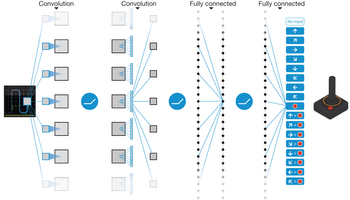
\includegraphics[width=442px,height=242px]{src/img/state/schematic-ilustration}
		\caption{Q-Network architecture\cite{nature}} \label{fig:arch}
    \end{center}
\end{figure}

The network is used to approximate the optimal action-value function $Q^{*}$\cite{nature}:
\begin{equation}
	Q^{*}(s,a) = \max_\pi E[r_t + \gamma\cdot r_{t+1} + \gamma^2\cdot r_{t+2} + \dotsc | s_t = s, a_t = a, \pi]
\end{equation}
The function Q is also parametrized with the weights and the agent state $e_t = (s_t,a_t,r_t,s_{t+1})$ is saved at each iteration in a set D_t = ${(e_1, e_2, \dotsc, e_t)}$
With all the necessary information here is the computation of the loss function\cite{nature}:

\begin{equation}
	L_i(\theta_i)=E_{(s,a,r,s^{\prime})}[(r + \gamma\cdot\max_{a^{\prime}}\cdot Q(s^{\prime},a^{\prime};{\theta_i}^-) - Q(s,a;\theta_i))^2]
\end{equation}

where $\gamma$ represents the discount factor and ${\theta_i}^-)$ is updated with $\theta_i$ every x defined steps and here is the gradient\cite{nature}:

\begin{equation}
\nabla_{\theta_i}L(\theta_i) = E_{s,a,r,{s^i}}[(r + \gamma\cdot\max_{a^{\prime}}Q(s^\prime, a^\prime;{\theta_i}^-)-Q(s,a;\theta_i))\nabla_{\theta_i}Q(s,a;\theta_i)]
\end{equation}

The Q-learning action-value function can be updates using ${\theta_i}^-$ = $\theta_{i-1}$ following the optimal policy with probability 1 - $\epsilon$ and selecting a random move with probability $\epsilon$. 

For minimizing the loss function, Stochastic Gradient Descent is used in combination with the experience replay technique for preventing `dead' neurons and also, Q is not updated at each iteration. This avoids the instability of Q caused by the nonlinearity of network.

The $\epsilon$-greedy policy was set to 0.05 and the Q-values were scaled because of big range values from rewards.
\newpage
\section{Algorithm}

One of the techniques that Q-Network algorithm is using is called experience replay. This implies transitions between states to be stored. A number of N transitions (the previous state, the current state, reward and action) are stored in a pool of transitions. Until the network starts learning, we have to play many episodes. We begin from initializing the pool where we store the experiences and initialize two different networks(action-value network Q and target action-value network $Q^-$) with the same weights. For each episode we start by storing the current transition which at first will be composed by only one state. With probability $\epsilon$ we choose a random action and with probability $1-\epsilon$ we choose the best action. After that, we apply the action on the current state of the game and observe reward and new state of the game. We put it in the pool and randomize it. The target value is the reward if game is finished or the sum between the reward observed and maxim-value predicted by target action-value $Q^-$ multiplied with the discount factor. Then we propagate the error as the mean squared error between target value and action-value function Q. Once \textbf{x} steps had pass we update the weights of $Q^-$ with the weights of Q. The algorithm\cite{atari} used for training Q-Network is presented as it follows:

\begin{algorithm}
	\floatname{algorithm}{Algorithm}
	\caption{Q-Network} \label{sgd-code}
	\begin{algorithmic}[1]
		\State create replay memory D for storing N experiences
		\State choose $\epsilon$ between (0,1)
		\State init Q model weights with $\theta$
		\State save $Q^-$ model weights to $\theta^-$
		\State init variable episode to 0 and choose MAX_EPISODES
		\While{episode < MAX_EPISODES}{
			\State generate state $s_1$ from frame: $s_1$ = {$image_1$}
			\While{game not over}
				\State r = random number between (0,1)
				\If{r < $\epsilon$}
					\State $a_t$ = random action
				\Else
					\State $a_t$ = $argmax_a$ Q($s_t$, a; $\theta$)
				\EndIf

				\State $s_{t+1}$ = ($s_t$,$a_t$,$image_{t+1}$)

				\State D = D + \{($s_t$, $a_t$, $r_t$, $s_{t+1}$)\}

				\State shuffle D

				\State extract ($s_j$, $a_j$, $r_j$, $s_{j+1}$) from D

				\If{episode is finished at step j+1}
					\State $y_j$ = $r_j$
				\Else
					\State $y_j$ = $r_j$ + $\gamma\cdot\max_{a^{\prime}}\cdot {Q^-}(s_{j+1},a^{\prime};\theta^-)$
				\EndIf
				\State propagate error $(y_j - Q(s_j,a_j;\theta))^2$
				\State at each \textbf{x} steps save model weights $\theta$ to $\theta^-$
			\EndWhile
		}\EndWhile

		
	\end{algorithmic}
\end{algorithm}

\newpage


\section{Results}

Q-Network is capable of learning the optimal policy. For example, in Breakout what is being learned is to make a tunnel between blocks in order to send the ball into the back. Receiving only the pixel from the frames, rewards and using the same network structure it is capable of playing different games. The Q-Network can achieve 75\% of a score of a human test at 49 games\cite{nature}. The games where the algorithm performs poorly are the games where the memory is needed. For example, on Montezuma's Revenge\footnote{\url{https://atariage.com/software_page.php?SoftwareID=1158}} we go from room to another rooms so it is very hard for the algorithm taking into account multiple scenarios changing instead of only one changing. Below there are the results for different types of games from Atari compared to the results of a professional human tester.


\begin{figure}[h]
	\floatname{algorithm}{Algorithm}
	\begin{center}
		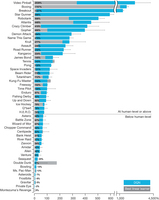
\includegraphics[width=367px,height=435px]{src/img/state/comparision}
		\caption{Comparison\cite{nature}} \label{fig:comp}
    \end{center}
\end{figure}




